\documentclass[a4paper,12pt]{article}
%\documentclass[a4paper,10pt]{scrartcl}

\usepackage[utf8]{inputenc}
\usepackage{mathptmx}
\usepackage[margin=2.5cm, includefoot]{geometry}
\usepackage{amsfonts, amsmath, amssymb}
\usepackage{graphicx}
\usepackage{float}
\usepackage{setspace}
\usepackage{titlesec}
\usepackage{hyperref}
\usepackage{url}
\usepackage{caption}
\usepackage{fancyhdr}
\usepackage{indentfirst}
\usepackage{etoolbox}
\AtBeginEnvironment{align}{\setcounter{equation}{0}}
% Header And Footer stuff
\pagestyle{fancy}
\fancyhead{}
\fancyfoot{}
\fancyfoot[R]{ \thepage\ }
\renewcommand{\headrulewidth}{1pt}
\renewcommand{\footrulewidth}{1pt}
%
\renewcommand*\contentsname{Daftar Isi}
\captionsetup[figure]{name=Gambar}

\onehalfspacing
\titleformat{\section}{\Large\normalfont\bfseries\filcenter}{\thesection.}{0.8em}{}
\titleformat{\subsection}{\large\normalfont\bfseries}{\thesubsection}{0.8em}{}
\renewcommand{\thesection}{\arabic{section}}
\hypersetup{
    colorlinks=true,
    linkcolor=blue,
    urlcolor=blue
}
\urlstyle{rm}

\title{}
\author{}
\date{}

\pdfinfo{%
  /Title    ()
  /Author   ()
  /Creator  ()
  /Producer ()
  /Subject  ()
  /Keywords ()
}

\begin{document}
\begin{titlepage}
\begin{center}
 \textbf{Write Up}
 \vspace{1cm}
\end{center}
\begin{figure}[H]
 \centering

\includegraphics[width=0.5\textwidth]{its}\\
\end{figure}
\vspace{3cm}
\begin{center}
\line(1,0){300}

\textbf{PicoCTF 2019}


Institut Teknologi Sepuluh Nopember
\\[1cm]
Aaron Christopher Tanhar

07211940000055

Dibuat menggunakan \LaTeX\

\line(1,0){300}\\
\end{center}
\end{titlepage}
\tableofcontents
\thispagestyle{empty}
\cleardoublepage
\setcounter{page}{1}
 \section{\textbf{plumbing(200 points)}}
\vspace{1cm}
Soal:
Sometimes you need to handle process data outside of a file. Can you find a way to keep the output from this program and search for the flag? Connect to 2019shell1.picoctf.com 57911.\\
Solusi:\\
nc 2019shell1.picoctf.com 57911 | grep "picoCTF\{.*\}"\\
EZ PZ
\section{\textbf{picobrowser(200 points)}}
\vspace{1cm}
Soal: This website can be rendered only by picobrowser, go and catch the flag! \\https://2019shell1.picoctf.com/problem/32205/ (link) or http://2019shell1.picoctf.com:32205\\
Solusi: Dari soalnya sendiri sudah memberi hint bahwa hanya user agent 'picobrowser' yang akan memberi flagnya.\\
curl -s -H "User-Agent: picobrowser" https://2019shell1.picoctf.com/problem/32205/flag | grep -oE "picoCTF\{.*\}"
\\
\section{\textbf{like1000(250 points)}}
\vspace{1cm}
Soal: This .tar file got tarred alot. \\
Solusi: Ketika kita mendownload file yang diberikan, akan didapati file berekstensi tar bernama 1000.tar\\
Ketika kita mengekstrak 1000.tar, akan didapati 999.tar. Maka hal ini akan sangat mudah apabila menggunakan script.
\begin{figure}[H]
 \centering
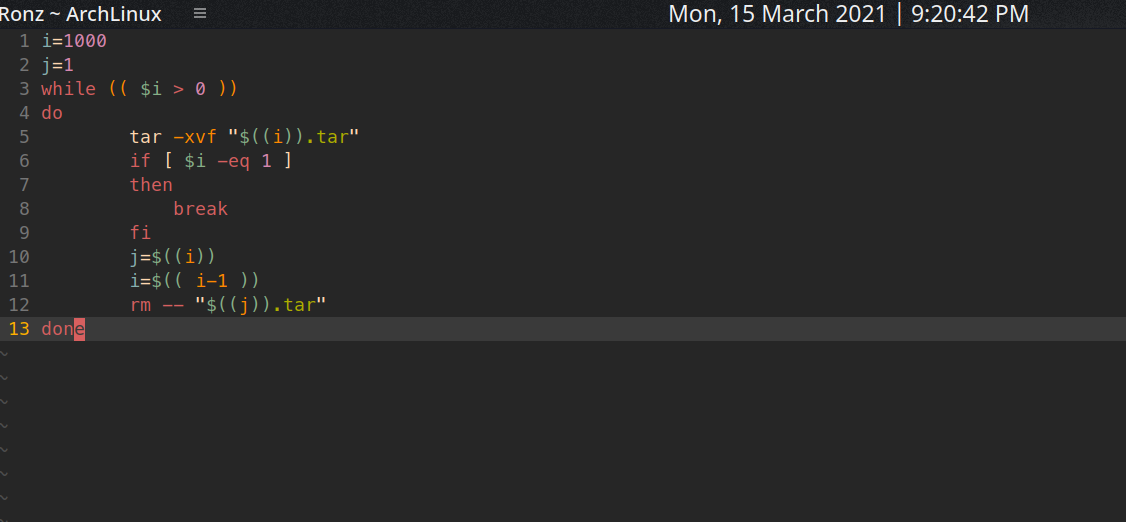
\includegraphics[width=1\textwidth]{like1000script.png}\\
\caption{Script yang digunakan}
\end{figure}
Ketika sudah mencapai 1.tar, ketika diekstrak akan muncul file png bernama flag.png
\begin{figure}[H]
 \centering
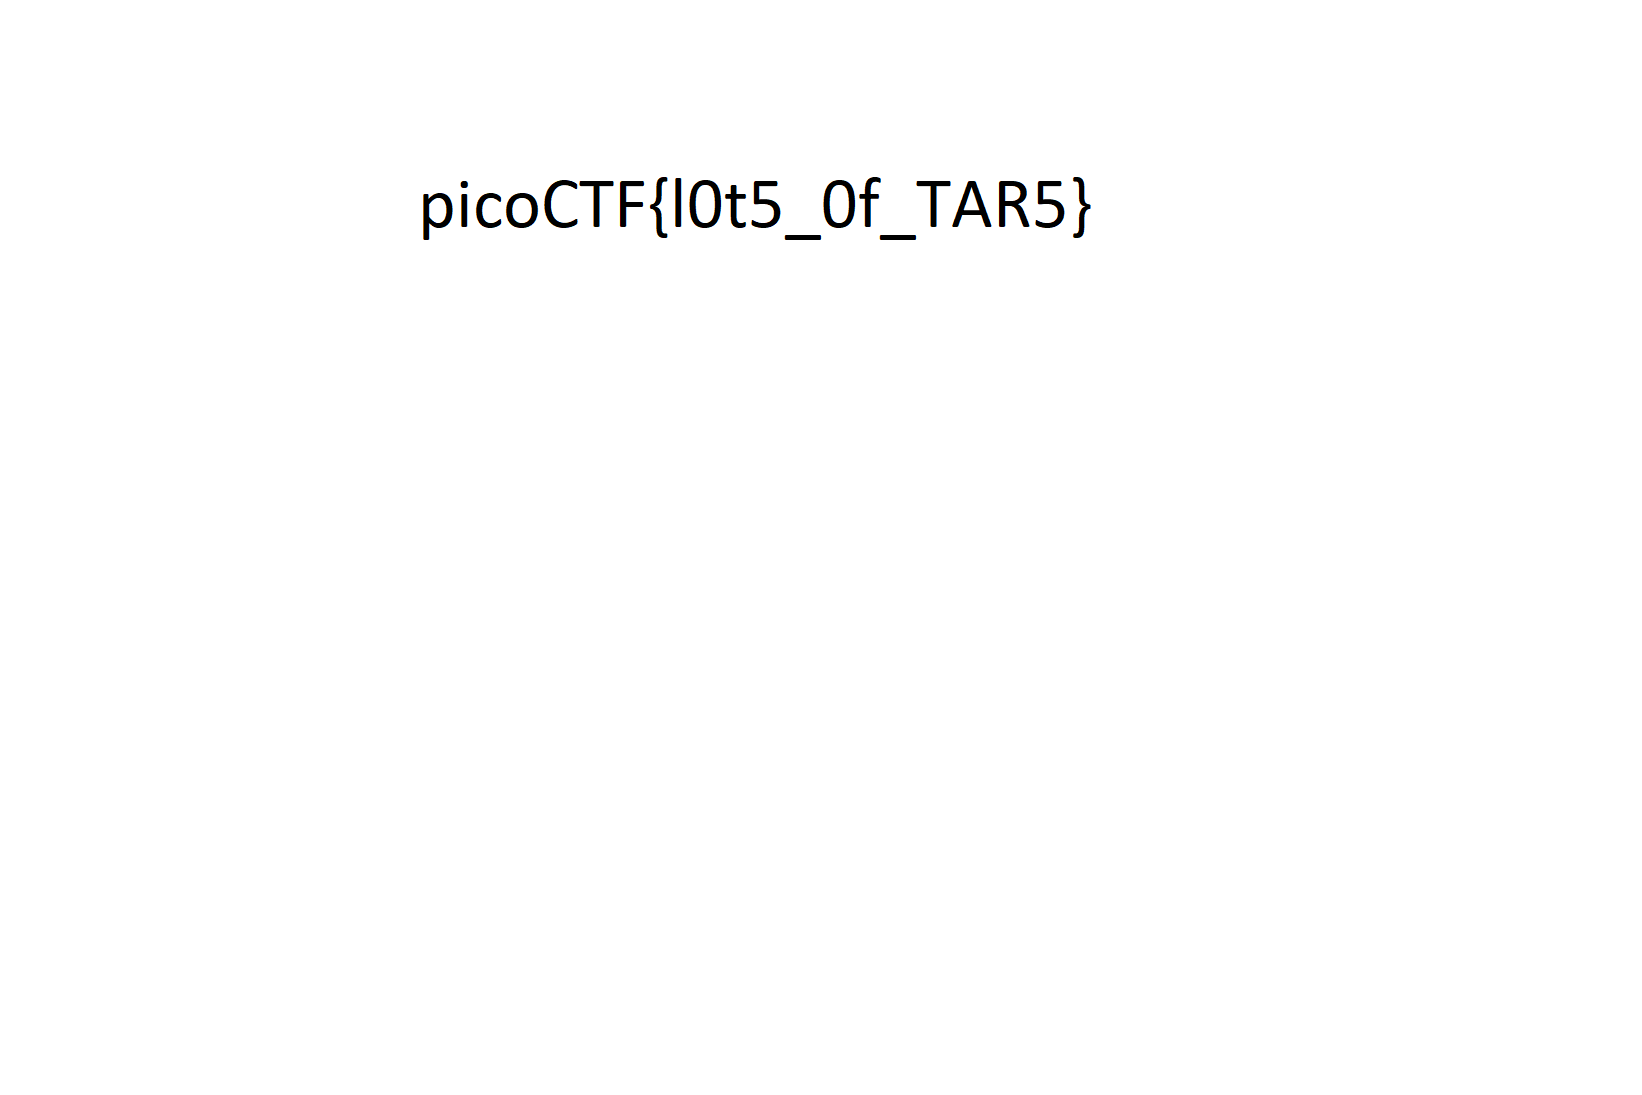
\includegraphics[width=0.7\textwidth]{like1000flag.png}\\
\caption{Flagnyaa}
\end{figure}
\section{\textbf{where-is-the-file(200 points)}}
Soal: I've used a super secret mind trick to hide this file. Maybe something lies in /problems/where-is-the-file\_6\_8eae99761e71a8a21d3b82ac6cf2a7d0.
Solusi:
Login ke shell picoCTF, lalu cd ke direktori yang ada di soal
Mudah sebenarnya, tinggal ls -a lalu cat saja
\begin{figure}[H]
 \centering
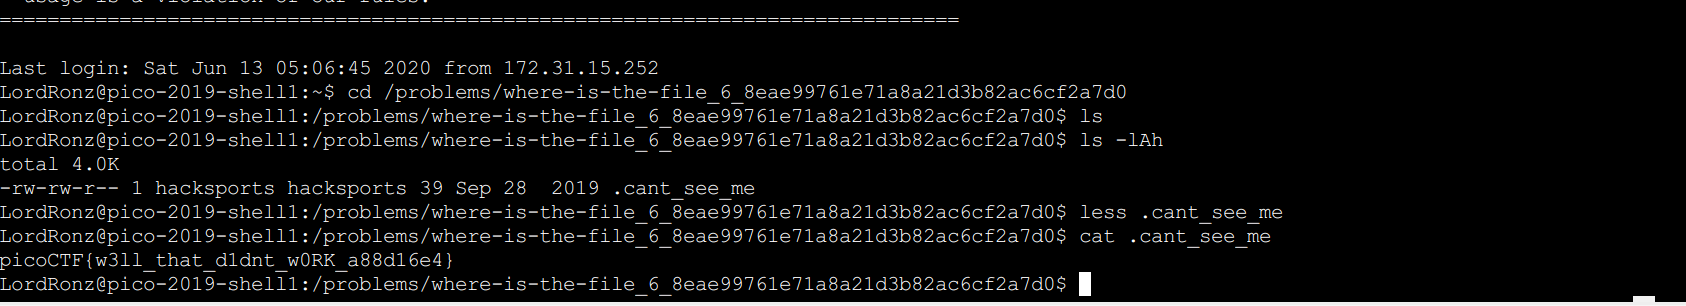
\includegraphics[width=1\textwidth]{wherefileflag.png}\\
\caption{Flagnyaa}
\end{figure}
\vspace{1cm}
\section{\textbf{open-to-admins(200 points)}}
Soal: This secure website allows users to access the flag only if they are admin and if the time is exactly 1400.\\ https:\/\/2019shell1.picoctf.com\/problem\/49858\/ (link) or http:\/\/2019shell1.picoctf.com:49858
Solusi: Dari soalnya dan hintnya bisa disimpulkan bahwa akan ada manipulasi cookie disini. Kita dapat mengganti cookie dengan console dan memberi value cookie ke variable document.cookie
\begin{figure}[H]
 \centering
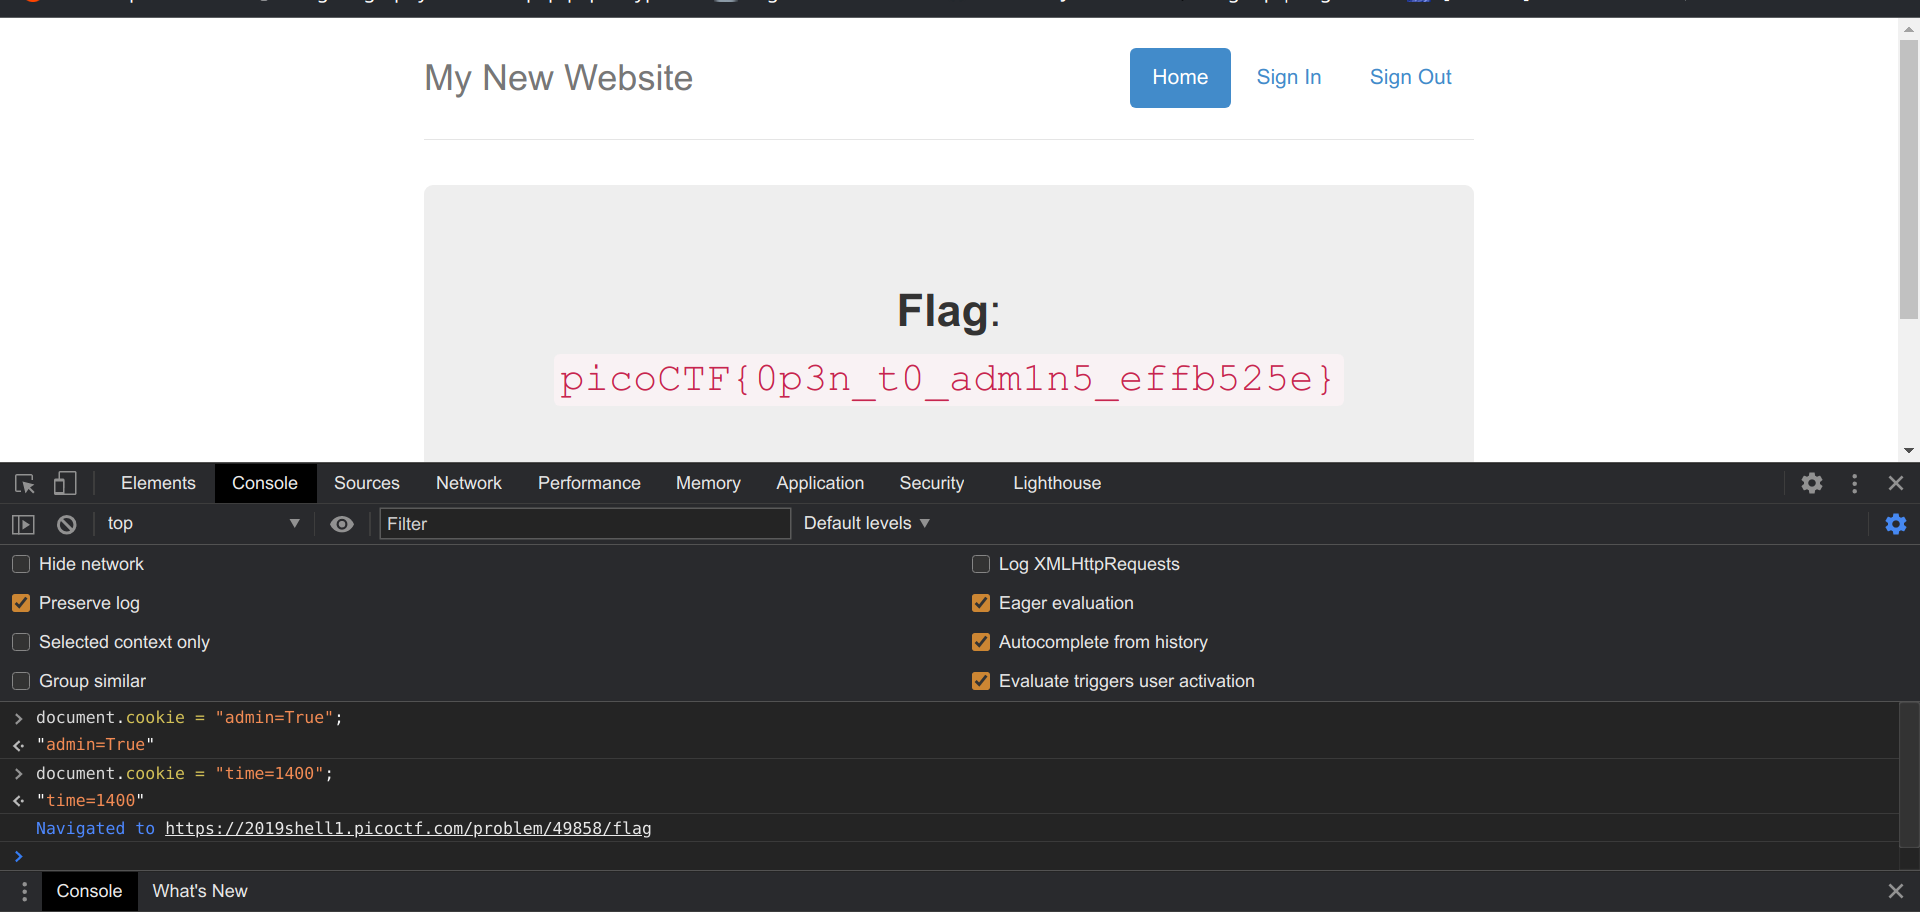
\includegraphics[width=1\textwidth]{opentoadminsflag.png}\\
\caption{Flagnyaa}
\end{figure}
\vspace{1cm}
\section{\textbf{flag\_shop(300 points)}}
Soal: There's a flag shop selling stuff, can you buy a flag? Source. Connect with nc 2019shell1.picoctf.com 63894.
Solusi: sebenarnya ini merupakan soal yang cukup mudah, karena kita diberi source codenya. Tipe int pada C maksimal menampung 2 pangkat 32 sehingga jika overflow maka nilainya akan minus.
\begin{figure}[H]
 \centering
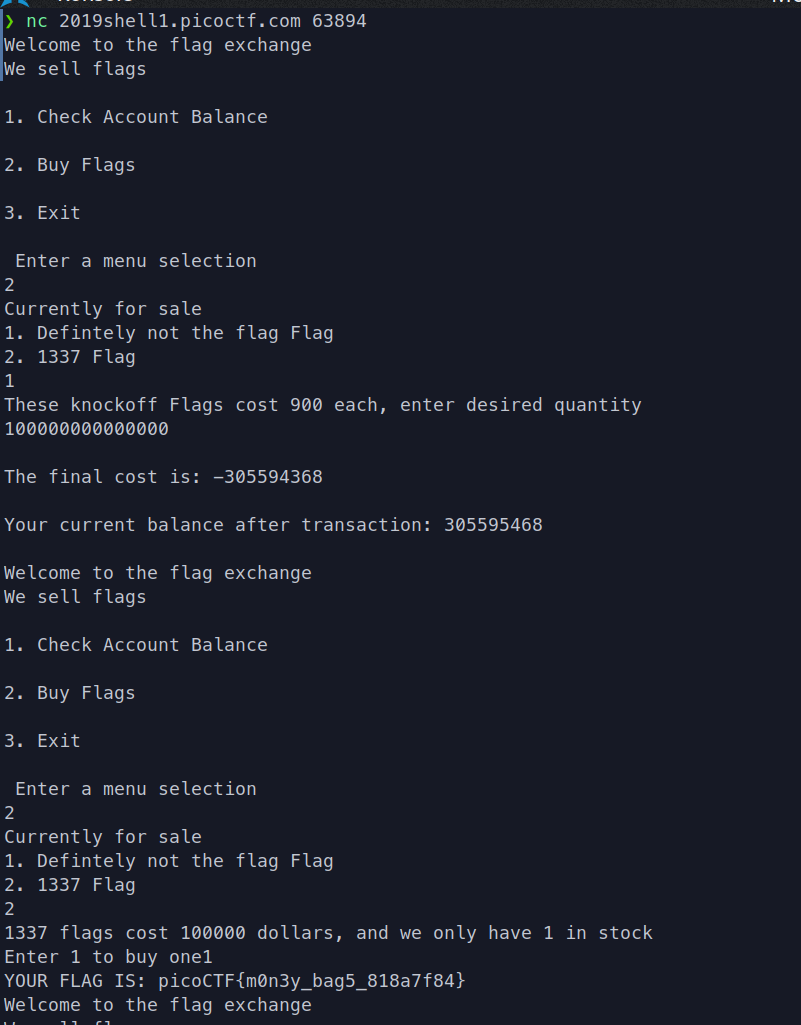
\includegraphics[width=1\textwidth]{flagshopflag.png}\\
\caption{Flagnyaa}
\end{figure}
\section{\textbf{JaWT Scratchpad(400 points)}}
Soal: Check the admin scratchpad! https:\/\/2019shell1.picoctf.com\/problem\/12283\/ or\\ http:\/\/2019shell1.picoctf.com:12283\\
Solusi: dari judulnya sudah dapat diterka bahwa problem ini akan berkaitan dengan JWT atau JSON web token.
\begin{figure}[H]
 \centering
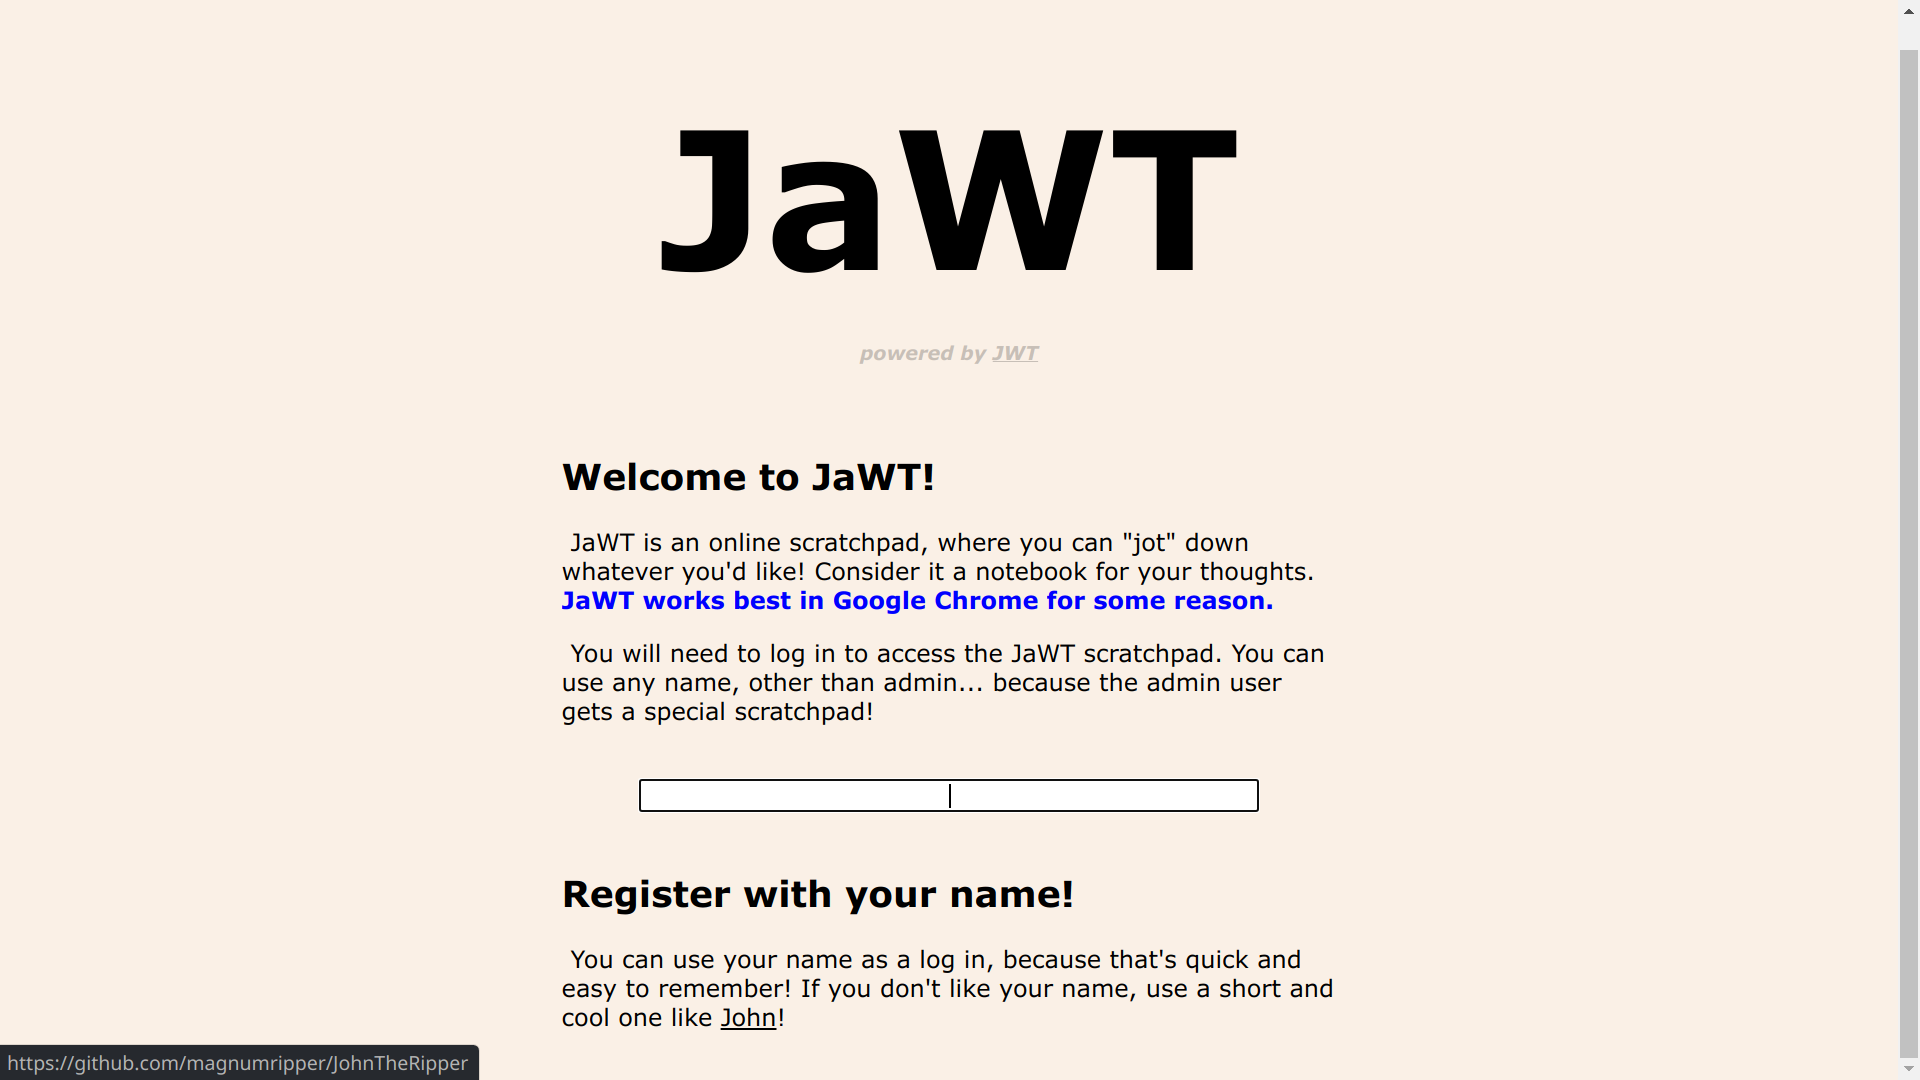
\includegraphics[width=1\textwidth]{jwtscratch1.png}\\
\caption{Tampilan dari link yang diberikan}
\end{figure}
Jika kita login dengan nama admin, maka tidak bisa dilakukan. Maka kita coba dengan mengisikan nama sembarang. Lalu kita bisa mengakses jwt.io untuk info lebih lengkap terkait JWT ini.
\begin{figure}[H]
 \centering
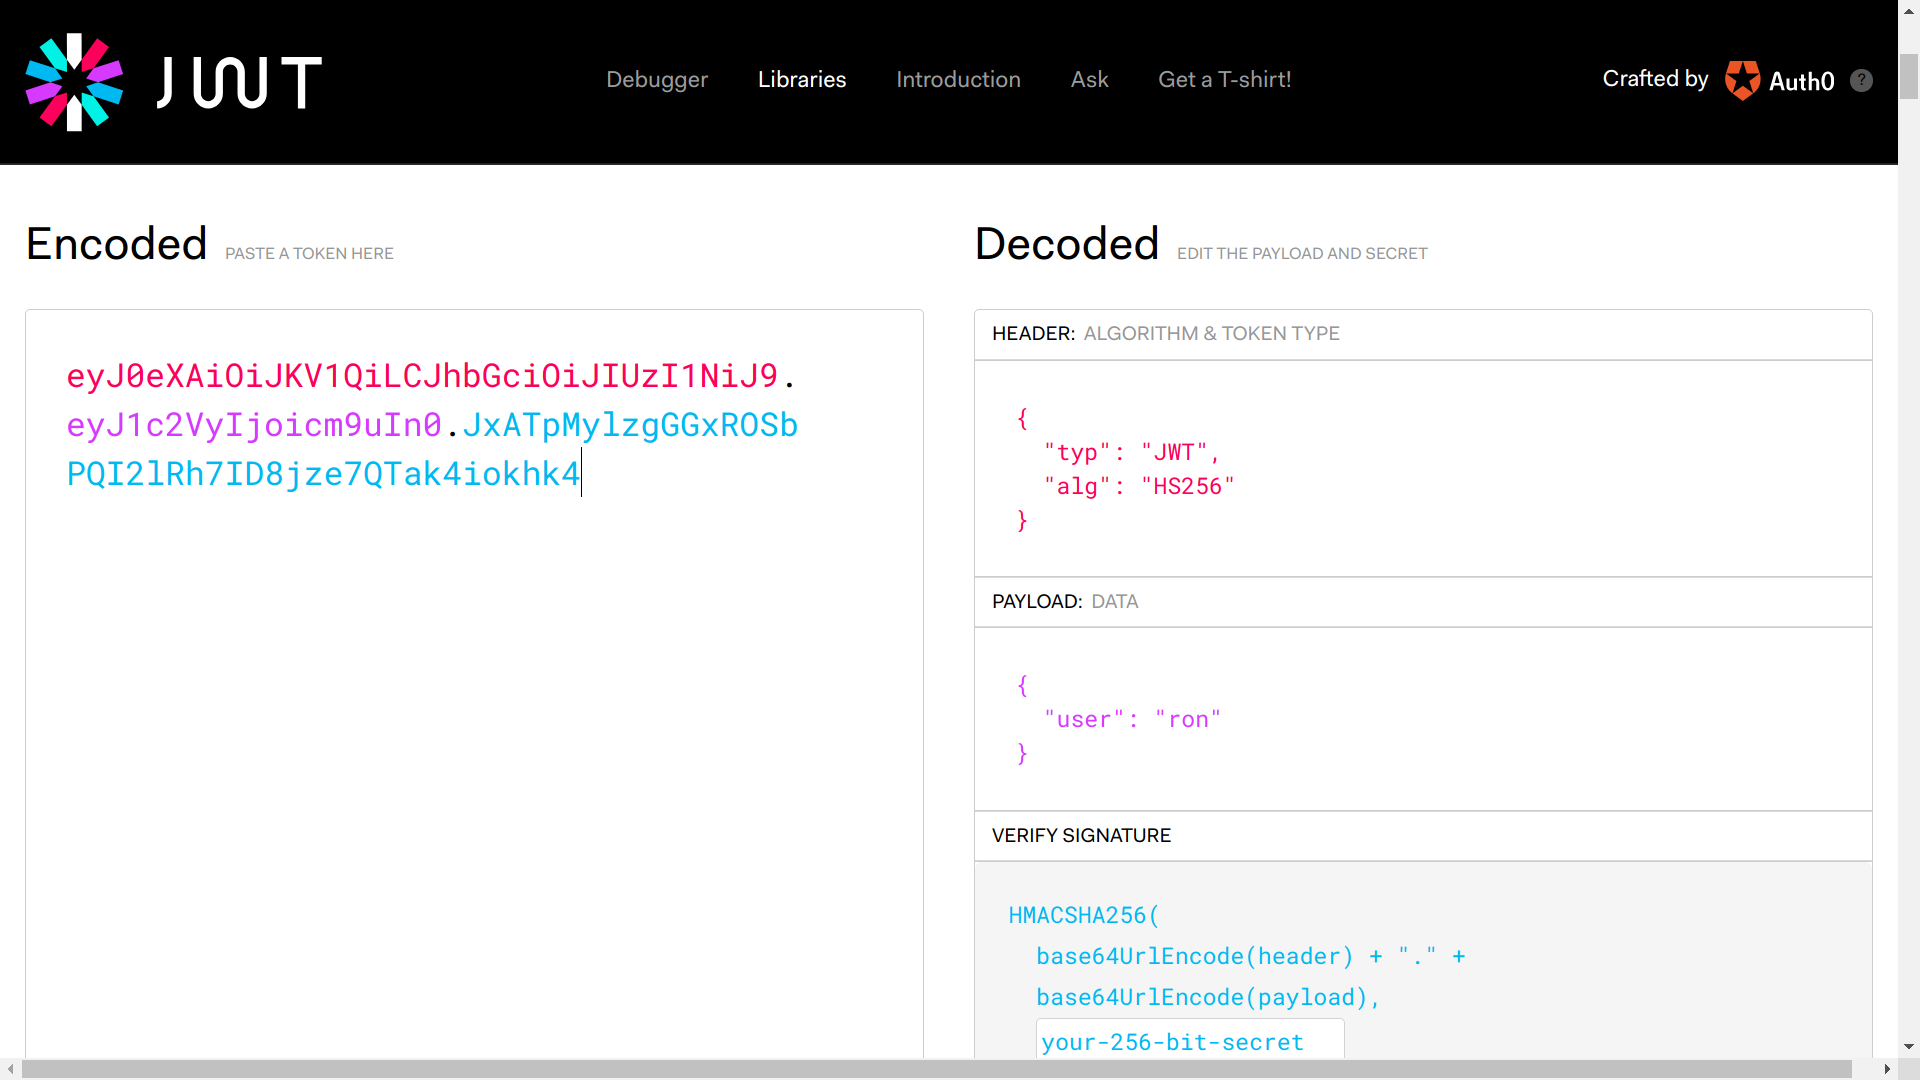
\includegraphics[width=1\textwidth]{jwtscratch2.png}\\
\caption{jwt.io}
\end{figure}
Dapat dilihat bahwa digunakan algoritma HS256. Lalu jika kita memperhatikan laman dari JaWT tadi ada hyperlink ke tools bernama John the Ripper, password cracker. picoCTF memberikan clue pada kita bahwa kita dapat menggunakan john the ripper untuk mengcrack problem ini.
Saya sudah memiliki wordlist bernama rockyou yang berukuran 130 mb.
\begin{figure}[H]
 \centering
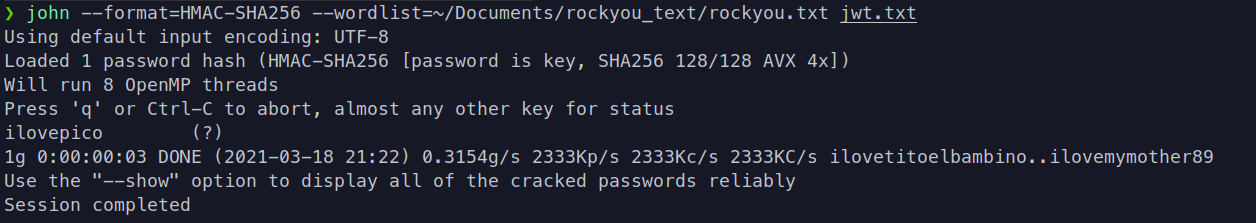
\includegraphics[width=1\textwidth]{jwtscratch3.png}\\
\caption{penggunaan john}
\end{figure}
Diperoleh secret keynya adalah ilovepico, maka kita tinggal mengubahnya dari jwt.io saja.
\begin{figure}[H]
 \centering
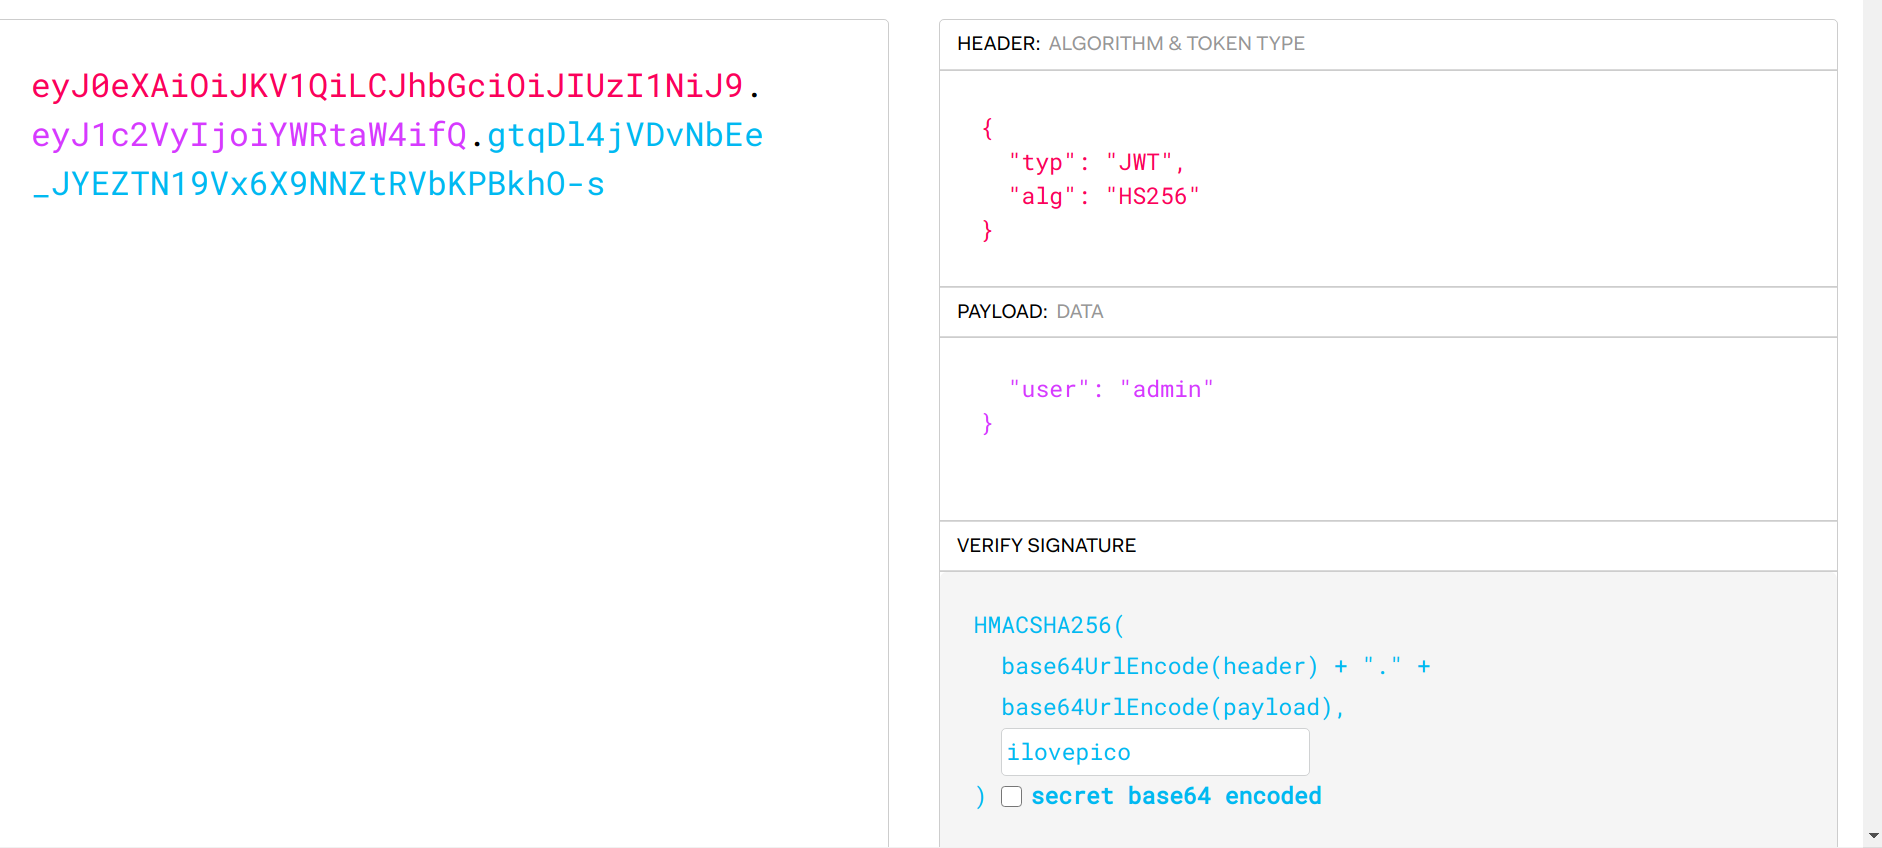
\includegraphics[width=1\textwidth]{jwtscratch4.png}\\
\caption{secret key diperoleh}
\end{figure}
Lalu kita tinggal mengatur cookie dari webpagenya tadi saja, maka akan terlihat flagnya.
\begin{figure}[H]
 \centering
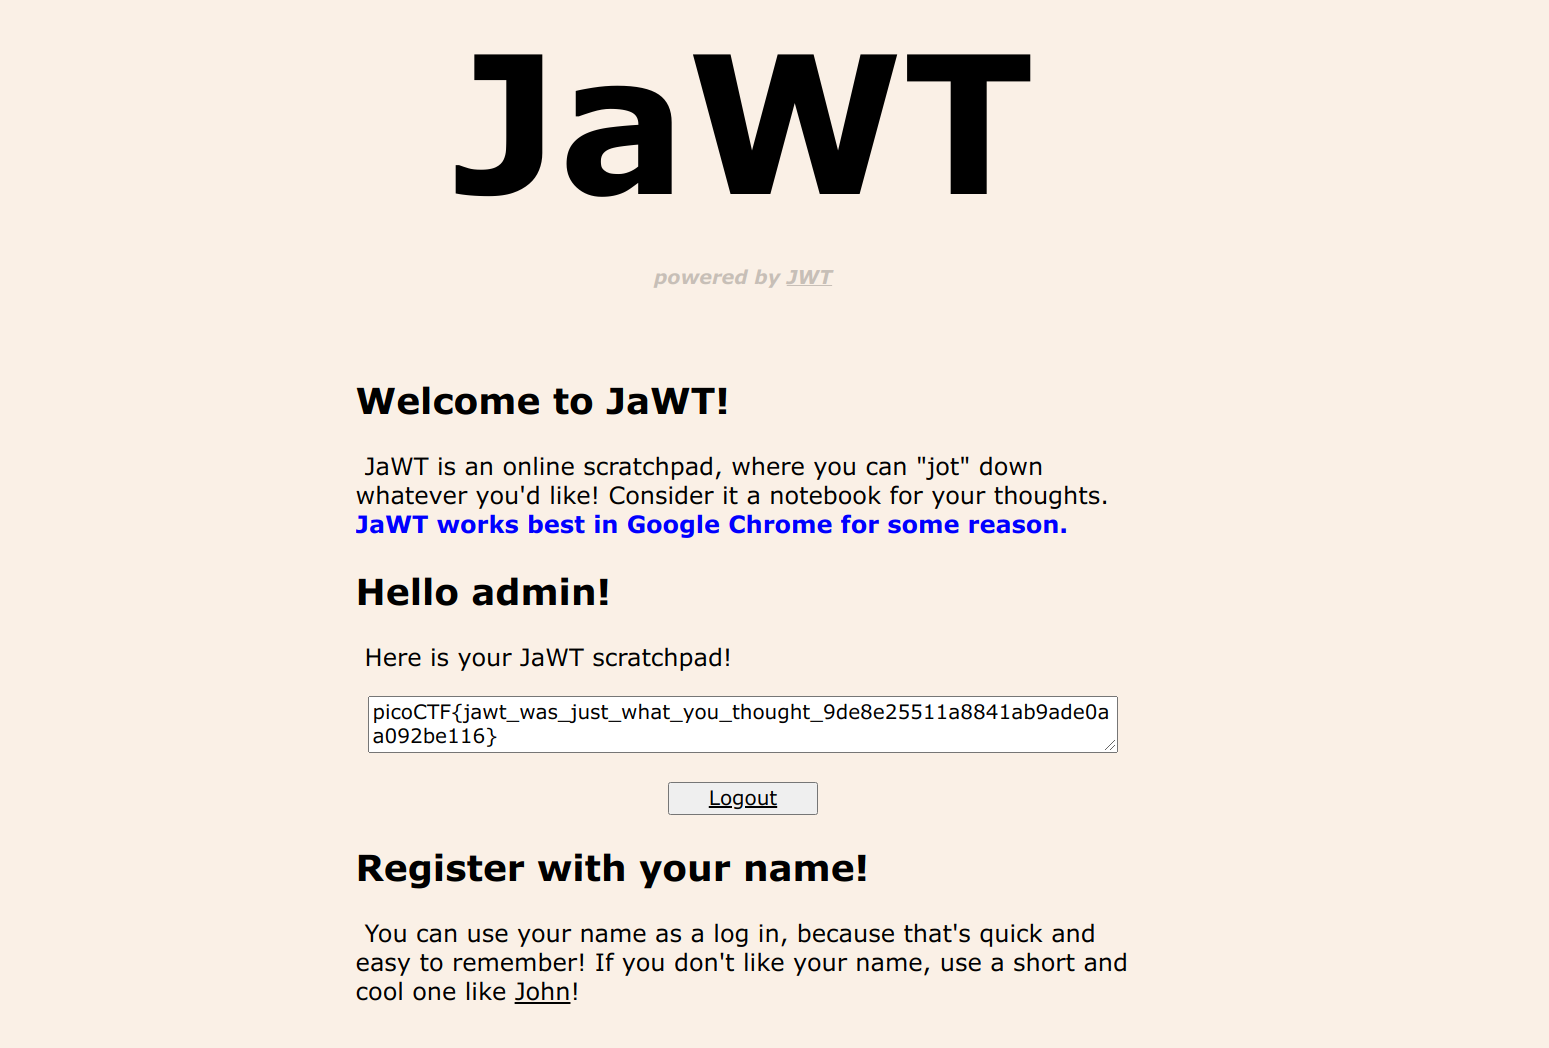
\includegraphics[width=1\textwidth]{jwtscratchflag.png}\\
\caption{Flagnyaa}
\end{figure}
\end{document}
